% GAN: the generator maps noise to samples; the discriminator scores real and generated
% samples; two alternating losses update phi and theta, and only G is kept for sampling.
\documentclass[border=0pt]{standalone}
\usepackage{amsmath,amssymb}
% Shared visual language for the figures of the book.
% Every figure in this directory loads this file so the chapter reads as one system.
% NOTE: no blank lines are allowed inside \tikzset{...} (a blank line emits \par
% and breaks key scanning).
\NeedsTeXFormat{LaTeX2e}
\ProvidesPackage{figstyle}[2026/10/21 Figure style for Free Energy to LLMs]

\RequirePackage{tikz}
\usetikzlibrary{arrows.meta,positioning,calc,fit,shapes.geometric,shapes.misc,%
  backgrounds,matrix,decorations.pathreplacing,decorations.markings,patterns.meta}

% ---------------------------------------------------------------- palette
% Same values as book/preamble/style.tex, prefixed with F.
\definecolor{FNavy}{HTML}{14324A}
\definecolor{FTeal}{HTML}{0E7490}
\definecolor{FSky}{HTML}{E7F5F8}
\definecolor{FOrange}{HTML}{D97706}
\definecolor{FAmber}{HTML}{FFF3D6}
\definecolor{FInk}{HTML}{1F2937}
\definecolor{FSlate}{HTML}{64748B}
\definecolor{FMist}{HTML}{F5F7FA}
\definecolor{FRose}{HTML}{9F1239}
\definecolor{FRoseMist}{HTML}{FFF1F2}

% ---------------------------------------------------------------- semantics
% Teal   = probability / model / data object
% Orange = training objective, cost, or the quantity moved through the system
% Navy   = neutral structure
% Slate  = secondary label or metadata
% Rose   = failure mode, hazard, masked-out region
\tikzset{
  % Lay figures out in millimetres.  A figure designed 168mm wide is included at
  % \textwidth, so its fonts appear at exactly the size written here.
  every picture/.style={x=1mm,y=1mm,font=\small,line cap=round,line join=round},
  % ---- block styles
  nbase/.style={draw,rounded corners=1.2pt,align=center,inner sep=2.4pt,%
    minimum height=7mm,text=FInk},
  nteal/.style={nbase,draw=FTeal,fill=FSky},
  norange/.style={nbase,draw=FOrange,fill=FAmber},
  nnavy/.style={nbase,draw=FNavy,fill=white},
  nsoft/.style={nbase,draw=FSlate!55,fill=FMist},
  nrose/.style={nbase,draw=FRose,fill=FRoseMist},
  ghost/.style={draw=none,fill=none,align=center,inner sep=1pt},
  plain/.style={draw=none,fill=none,align=center,inner sep=0pt},
  % ---- arrows
  ar/.style={-{Latex[length=1.7mm,width=1.35mm]},draw=FSlate,line width=0.75pt},
  ard/.style={ar,dashed},
  arteal/.style={ar,draw=FTeal},
  arorange/.style={ar,draw=FOrange},
  arrose/.style={ar,draw=FRose},
  thickar/.style={ar,line width=1.2pt},
  % ---- text roles
  ftitle/.style={font=\large\bfseries,text=FNavy,align=center},
  ptitle/.style={font=\small\bfseries,text=FNavy,align=center},
  ptitleo/.style={font=\small\bfseries,text=FOrange,align=center},
  lbl/.style={font=\scriptsize,text=FSlate,align=center,inner sep=1pt},
  lblt/.style={lbl,text=FTeal},
  lblo/.style={lbl,text=FOrange},
  lbln/.style={lbl,text=FNavy},
  lblr/.style={lbl,text=FRose},
  sub/.style={font=\scriptsize,text=FSlate!90,align=center,inner sep=1pt},
  monob/.style={font=\ttfamily\scriptsize,text=FInk,inner sep=1pt},
  mathb/.style={font=\small,text=FInk,inner sep=1pt},
  eqn/.style={font=\scriptsize,inner sep=1.5pt,text=FInk},
  % ---- decorations
  brace/.style={decorate,decoration={brace,amplitude=2.4pt},draw=FSlate,%
    line width=0.6pt},
  bracet/.style={brace,draw=FTeal},
  braceo/.style={brace,draw=FOrange},
  axis/.style={draw=FSlate!55,line width=0.6pt},
  guide/.style={draw=FSlate!45,line width=0.5pt,dashed},
  halolabel/.style={font=\scriptsize,text=FInk,fill=white,fill opacity=0.85,%
    text opacity=1,inner sep=1.4pt,align=center},
}

% Figure title above the drawing, anchored at the figure's top-left.
\newcommand{\figtitle}[2][0]{%
  \node[ftitle,anchor=north west,outer sep=0pt] at (#1,0) {#2};}

% Rounded panel behind a subgroup of nodes.
\newcommand{\figpanel}[3][]{%
  \node[draw=FSlate!35,fill=#3,rounded corners=2pt,inner sep=2.6mm,#1] {#2};}

\endinput

\begin{document}
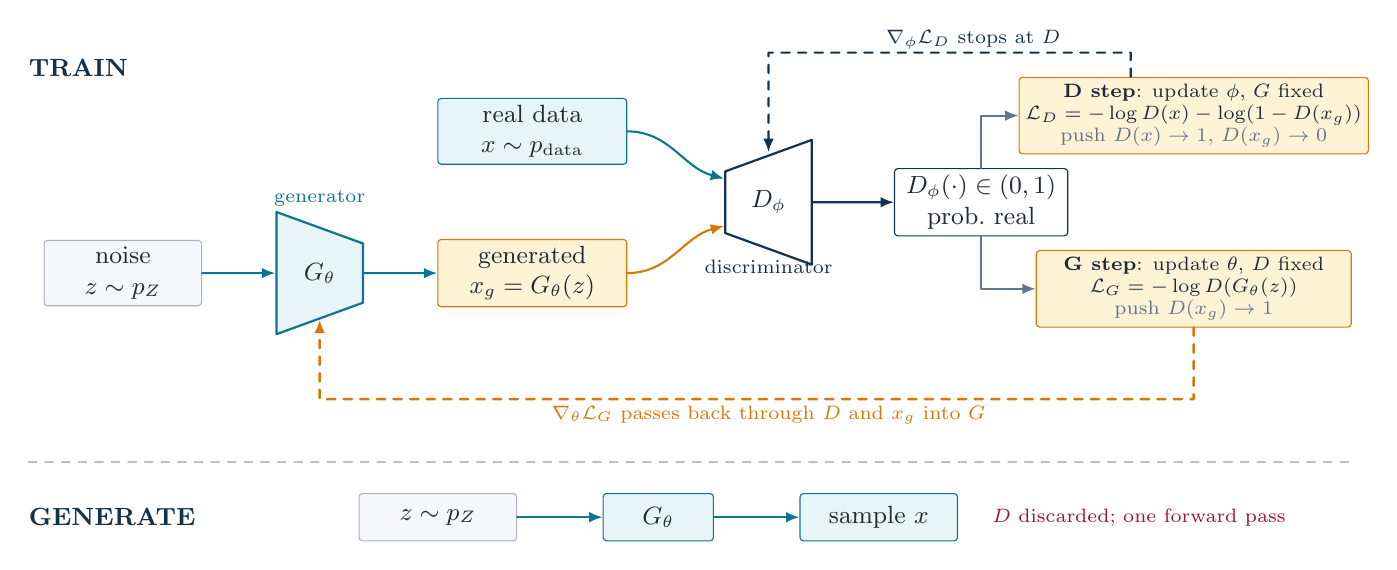
\begin{tikzpicture}
\node[plain,anchor=west,font=\small\bfseries,text=FNavy] at (0,56) {TRAIN};
% ------------------------------------------------------------------ generator path
\node[nsoft,minimum width=20mm] (z) at (12,30) {noise\\$z\sim p_Z$};
\node[trapezium,trapezium angle=70,shape border rotate=270,draw=FTeal,fill=FSky,line width=0.8pt,
  minimum height=11mm,minimum width=9mm,inner sep=1pt,align=center,text=FInk] (G) at (37,30) {$G_\theta$};
\node[lblt,anchor=south] at ($(G.north)+(0,2.2)$) {generator};
\node[norange,minimum width=24mm] (xg) at (64,30) {generated\\$x_g=G_\theta(z)$};
\draw[arteal] (z)--(G);
\draw[arteal] (G)--(xg);
% ------------------------------------------------------------------ real data
\node[nteal,minimum width=24mm] (xr) at (64,48) {real data\\$x\sim p_{\mathrm{data}}$};
% ------------------------------------------------------------------ discriminator
\node[trapezium,trapezium angle=70,shape border rotate=90,draw=FNavy,fill=white,line width=0.8pt,
  minimum height=11mm,minimum width=9mm,inner sep=1pt,align=center,text=FInk] (D) at (94,39) {$D_\phi$};
\node[lbln,anchor=north] at ($(D.south)+(0,-0.8)$) {discriminator};
\draw[arteal] (xr.east) to[out=0,in=165] ($(D.west)+(0,3)$);
\draw[arorange] (xg.east) to[out=0,in=195] ($(D.west)+(0,-3)$);
\node[nnavy,minimum width=22mm] (out) at (121,39) {$D_\phi(\cdot)\in(0,1)$\\prob.\ real};
\draw[ar,draw=FNavy] (D)--(out);
% ------------------------------------------------------------------ two losses
\node[norange,minimum width=40mm,font=\scriptsize] (LD) at (148,50) {\textbf{D step}: update $\phi$, $G$ fixed\\$\mathcal L_D=-\log D(x)-\log(1-D(x_g))$\\{\color{FSlate}push $D(x)\to1$, $D(x_g)\to0$}};
\node[norange,minimum width=40mm,font=\scriptsize] (LG) at (148,28) {\textbf{G step}: update $\theta$, $D$ fixed\\$\mathcal L_G=-\log D(G_\theta(z))$\\{\color{FSlate}push $D(x_g)\to1$}};
\draw[ar] (out.north) |- (LD.west);
\draw[ar] (out.south) |- (LG.west);
% ------------------------------------------------------------------ gradient paths
\draw[ard,draw=FNavy] ($(LD.north)+(-8,0)$) |- (94,58) -- ($(D.north)+(0,0.3)$);
\node[lbln,anchor=south] at (120,58) {$\nabla_\phi\mathcal L_D$ stops at $D$};
\draw[arorange,dashed,line width=0.9pt] (LG.south) |- (37,14) -- (G.south);
\node[lblo,anchor=north] at (94,13.6) {$\nabla_\theta\mathcal L_G$ passes back through $D$ and $x_g$ into $G$};
\draw[guide] (0,6) -- (168,6);
% ------------------------------------------------------------------ generation
\node[plain,anchor=west,font=\small\bfseries,text=FNavy] at (0,-1) {GENERATE};
\node[nsoft,minimum width=20mm,minimum height=6mm] (z2) at (52,-1) {$z\sim p_Z$};
\node[nteal,minimum width=14mm,minimum height=6mm] (G2) at (80,-1) {$G_\theta$};
\node[nteal,minimum width=20mm,minimum height=6mm] (x2) at (108,-1) {sample $x$};
\draw[arteal] (z2)--(G2);
\draw[arteal] (G2)--(x2);
\node[lblr,anchor=west] at (122,-1) {$D$ discarded; one forward pass};
\end{tikzpicture}
\end{document}
